\documentclass[a4paper,12pt]{article}
\usepackage{graphicx} % Required for inserting images
\usepackage[
    top=2.5cm,
    bottom=2.5cm,
    left=2.5cm,
    right=2.5cm
]{geometry}
\usepackage{tikz}
\usetikzlibrary{arrows.meta}
\usepackage{enumitem}
\usepackage{amssymb}
\usepackage{amsmath}


\newlist{questions}{enumerate}{2}
\setlist[questions,1]{
    label=\arabic*.,
    align=left,
    leftmargin=0pt,
    listparindent=\parindent,
    labelwidth=0pt,
    itemindent=!
}
\setlist[questions,2]{
    label=\arabic{questionsi}.\ \alph*),
    align=left,
    leftmargin=0pt,
    listparindent=\parindent,
    labelwidth=0pt,
    itemindent=!
}

\title{tfjm$^{2}$ 2027}
\author{Equipe Lycée Rocroy Saint-Vincent de Paul}
\date{November 2026}

\begin{document}

\maketitle

\section{\sc{Chaises musicales au restaurant}}

\begin{questions}

\begin{figure}[ht]
\centering
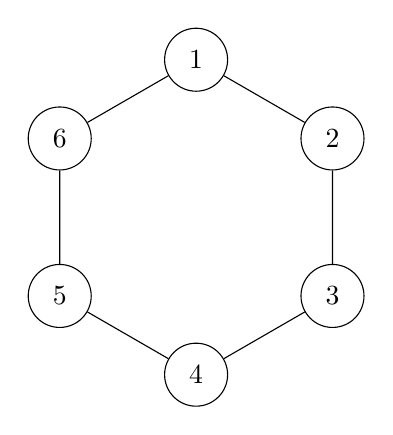
\begin{tikzpicture}[
    vertex/.style={
        circle,
        draw,
        minimum size=8mm,
        inner sep=0pt
    }
]

\foreach \i in {1,...,6} {
    \node[vertex] (\i) at ({90-60*(\i-1)}:2cm) {\i};
}

\draw (1) -- (2) -- (3) -- (4) -- (5) -- (6) -- (1);

\end{tikzpicture}
\quad
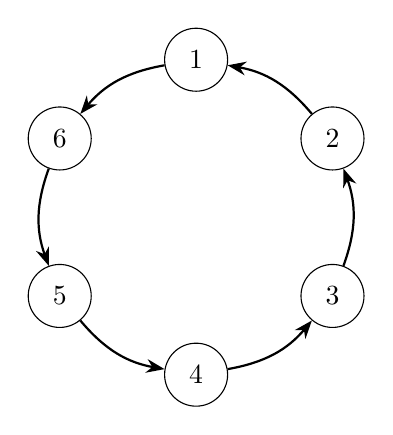
\begin{tikzpicture}[
    vertex/.style={
        circle,
        draw,
        minimum size=8mm,
        inner sep=0pt
    },
    arrow/.style={
        -{Stealth},
        thick,
        bend right=20
    }
]

\foreach \i in {1,...,6} {
    \node[vertex] (\i) at ({90-60*(\i-1)}:2cm) {\i};
}

\draw[arrow] (1) to (6);
\draw[arrow] (6) to (5);
\draw[arrow] (5) to (4);
\draw[arrow] (4) to (3);
\draw[arrow] (3) to (2);
\draw[arrow] (2) to (1);

\end{tikzpicture}
\caption{n=6, table ronde, plan de table et consigne de rotation}
\label{fig1.a}
\end{figure}

    \stepcounter{questionsi}\item[]
    \begin{questions}
    \item
    Le plan de table est invariant par rotation. Lorsque le plat $1<i\leq 10$ est servi, deux convives sont assis à deux places reliées si et seulement si ils étaient assis à deux places reliées au plat précédent.

    ...

    \item
    Chaque convives ne peut parler qu'à deux personnes différentes par plat. Pour que chaque convive puisse parler aux cinq autres personnes présentes il faudra nécessairement 3 plats.

    La figure \ref{fig1.b} représente (à faire !) un exemple de consigne de rotation qui réalise le minimum de 3 plats (à démontrer !).

    \begin{figure}[ht]
    \centering
        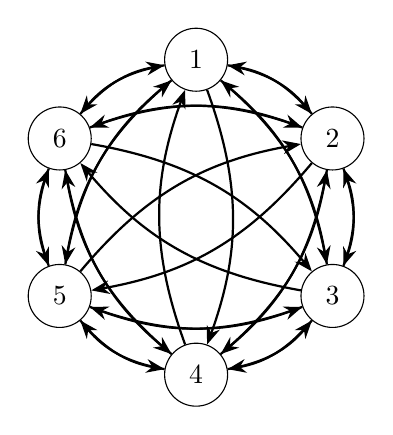
\begin{tikzpicture}[
        vertex/.style={
            circle,
            draw,
            minimum size=8mm,
            inner sep=0pt
        },
        arrowr/.style={
            -{Stealth},
            thick,
            bend right=20
        },
        arrowl/.style={
            -{Stealth},
            thick,
            bend left=20
        }
        ]
            
            \foreach \i in {1,...,6} {
                \node[vertex] (\i) at ({90-60*(\i-1)}:2cm) {\i};
            }
            
        \draw[arrowl] (1) to (2);
        \draw[arrowl] (1) to (3);
        \draw[arrowl] (1) to (4);
        \draw[arrowr] (1) to (5);
        \draw[arrowr] (1) to (6);
        \draw[arrowr] (2) to (1);
        \draw[arrowl] (2) to (3);
        \draw[arrowl] (2) to (4);
        \draw[arrowl] (2) to (5);
        \draw[arrowr] (2) to (6);
        \draw[arrowr] (3) to (2);
        \draw[arrowl] (3) to (4);
        \draw[arrowl] (3) to (5);
        \draw[arrowl] (3) to (6);
        \draw[arrowr] (3) to (1);
        \draw[arrowr] (4) to (3);
        \draw[arrowl] (4) to (5);
        \draw[arrowl] (4) to (6);
        \draw[arrowl] (4) to (1);
        \draw[arrowr] (4) to (2);
        \draw[arrowr] (5) to (4);
        \draw[arrowr] (5) to (3);
        \draw[arrowl] (5) to (2);
        \draw[arrowl] (5) to (6);
        \draw[arrowl] (5) to (1);
        \draw[arrowl] (6) to (1);
        \draw[arrowl] (6) to (2);
        \draw[arrowl] (6) to (3);
        \draw[arrowr] (6) to (4);
        \draw[arrowr] (6) to (5);
\end{tikzpicture}
    \caption{Consigne de rotation permettant à chaque convive de parler à tout la monde après trois plats}
    \label{fig1.b}
    \end{figure}
    
    \end{questions}
    

\end{questions}

\section{\sc{Dés personnalisés}}

D'après l'exemple de l'énoncé l'espérance du dé de Léo est :
\begin{align*}
    \mathbb{E}(X_L) &= 1\times\frac{1}{6}+2\times\frac{1}{6}+3\times\frac{1}{6}+5\times\frac{1}{6}+8\times\frac{1}{6}+13\times\frac{1}{6} \\
     &= \frac{16}{3}.    
\end{align*}
Celle de Théo :
\begin{align*}
    \mathbb{E}(X_T) &= 0\times\frac{1}{4}+2\times\frac{1}{4}+10\times\frac{1}{4}+10\times\frac{1}{4}\\
     &= \frac{11}{2}.
\end{align*}

Le score de Léo est défini comme la probabilité que Léo tire un chiffre strictement plus grand que celui de Théo plus la moitié de celle que ces deux chiffres soient égaux :
$$
    S_L = P(X_L>X_T) + \frac{1}{2}P(X_l=X_T).
$$

L'application numérique dans le cas de l'exemple de l'énoncé est :
\begin{align*}
    S_T &= P(X_T>X_L\mid X_T=10)\times P(X_T=10) + P(X_T>X_L\mid X_T=2)\times P(X_T=2)\\
    &\quad + P(X_T>X_L\mid X_T=0)\times P(X_T=0) + \frac{1}{2}P(X_T=X_L\mid X_T=10)\times P(X_T=10)\\
    &\quad + \frac{1}{2}P(X_T=X_L\mid X_T=2)\times P(X_T=2) + \frac{1}{2}P(X_T=X_L\mid X_T=0)\times P(X_T=0)
\end{align*}
soit encore
\begin{align*}
    S_T &= P(10>X_L)\times P(X_T=10) + P(2>X_L)\times P(X_T=2)\\
    &\quad + P(0>X_L)\times P(X_T=0) + \frac{1}{2}P(10=X_L)\times P(X_T=10)\\
    &\quad + \frac{1}{2}P(2=X_L)\times P(X_T=2) + \frac{1}{2}P(0=X_L)\times P(X_T=0)\\
    &= \frac{5}{6}\times\frac{1}{2} + \frac{1}{6}\times\frac{1}{4} + 0 + 0 + \frac{1}{2}\times\frac{1}{6}\times\frac{1}{4} + 0\\
    &= \frac{23}{48}
\end{align*}
\begin{questions}
    \stepcounter{questionsi}\item[]
    \begin{questions}
    
    \item
    Le pire score pour Théo est...

    \item Le meilleur score pour Théo est...

    \end{questions}

\end{questions}

\section{\sc{La couturière de vérité}}

Partie de Louis...

\section{\sc{Triskaïdékaphobie}}

Partie d'Eloi...

\section{\sc{Perdus dans la forêt}}

Partie de Béline...

\end{document}
